\chapter{关键信息驱动的三维光场静态人脸光照编辑}

近年来，三维光场技术取得显著进步，三维光场显示可以提供理想的立体视觉体验，观者在其中观看三维场景就像它们存在于真实空间一样。它能够提升虚拟现实等领域的用户体验，对于数字媒体和人机交互的发展起到重要影响。真实空间中，物体的明暗分布取决于光照，光照与阴影可以凸显画面的深度。而在三维光场显示中，光照同样是增加 3D 显示真实感和空间感的重要因素，通过编辑光照，可以大大提升立体显示效果。而合理准确的光照对于三维光场的显示效果起到非常关键的作用，光照编辑是三维光场中用于调整三维光场显示效果的常用方法。目前，对于三维光场人像光照编辑有两种方式。分别是多视图同时编辑方法和基于光照条件的密集视点采集方法。

对于多视图同时编辑方法，由于三维光场内容由多视图构成，不同视图间的光照信息相互关联，当单独处理某一单张视图的光照时，会使多视图之间的光照一致性得不到保证,进而削弱三维光场的真实感与连贯性。对于基于光照条件的密集视点采集方法，可以保证较好的多视图之间的光照一致性，但是需要搭建大规模数据采集设备。

为解决三维光场人像编辑中面临的数据采集复杂与光照一致性问题，本章提出了一种关键信息驱动的三维光场人像光照编辑方法，该方法通过抽取三维光场的多视图，获取漫反射分量，针对抽取的单张人像图像，采用高光去除算法对原始光照进行预处理，结合高光阈值多重判断来去除图像高光。从全景 HDR 图像中快速获取环境光信息并使用语义级别描述\cite{Dong2016,Sennrich2016,Vaswani2017}的对光照潜空间的关键信息进行编辑，获取关键光照信息(SH系数)\cite{Google2025,Ramamoorthi2001}
。最后进行重建，将图像解耦成几何空间和光照潜空间\cite{Jiang2023}，然后通过体渲染\cite{Mildenhall2022}渲染得到多视图，最后通过光场编码后在3D显示器上进行显示验证，完成对三维光场人像光照的编辑。通过实验对本方法进行了客观和主观评价，在多项指标上均优于先前的重光照方法，证明了该方法在提高了光照一致性的前提下，简单高效的实现了对三维光场人像光照的编辑。



\section{基本原理}
对于三维光场人像光照的编辑，常常使用多张视差图同时进行光照编辑的方法和基于光照条件的密集视点采集方法。前者方法虽然简单，但是在三维光场背景下却不再适用。三维光场内容由多视图构成，不同视图间的光照信息相互关联，当分别编辑某单张视图的光照时，会使得编辑后的多视图之间的光照一致性得不到保证，进而导致三维光场的真实感与连贯性降低。后者方法保证光照的一致性，通过搭建密集光场采集设备，同时部署多组可独立调控的 LED 光源，分布在相机阵列外围或顶部，形成自定义光照条件来拍摄得到多视图。但是密集视点采集方法需要搭建大规模数据采集设备。

基于上述背景，为解决三维光场人像光照编辑中的光照一致性不强和采集方法复杂的问题。本文提出了一种关键信息驱动的三维光场人像光照编辑方法，通过获取图像中的光照关键信息，在提高了光照一致性的前提下，简单高效的实现了对三维光场光照的编辑，完整的工作流程图如图\ref{fig:3-1}所示。

\begin{figure}[htbp]
  \centering
  %\vspace{1 cm} % 使用该指令调整上下间距
  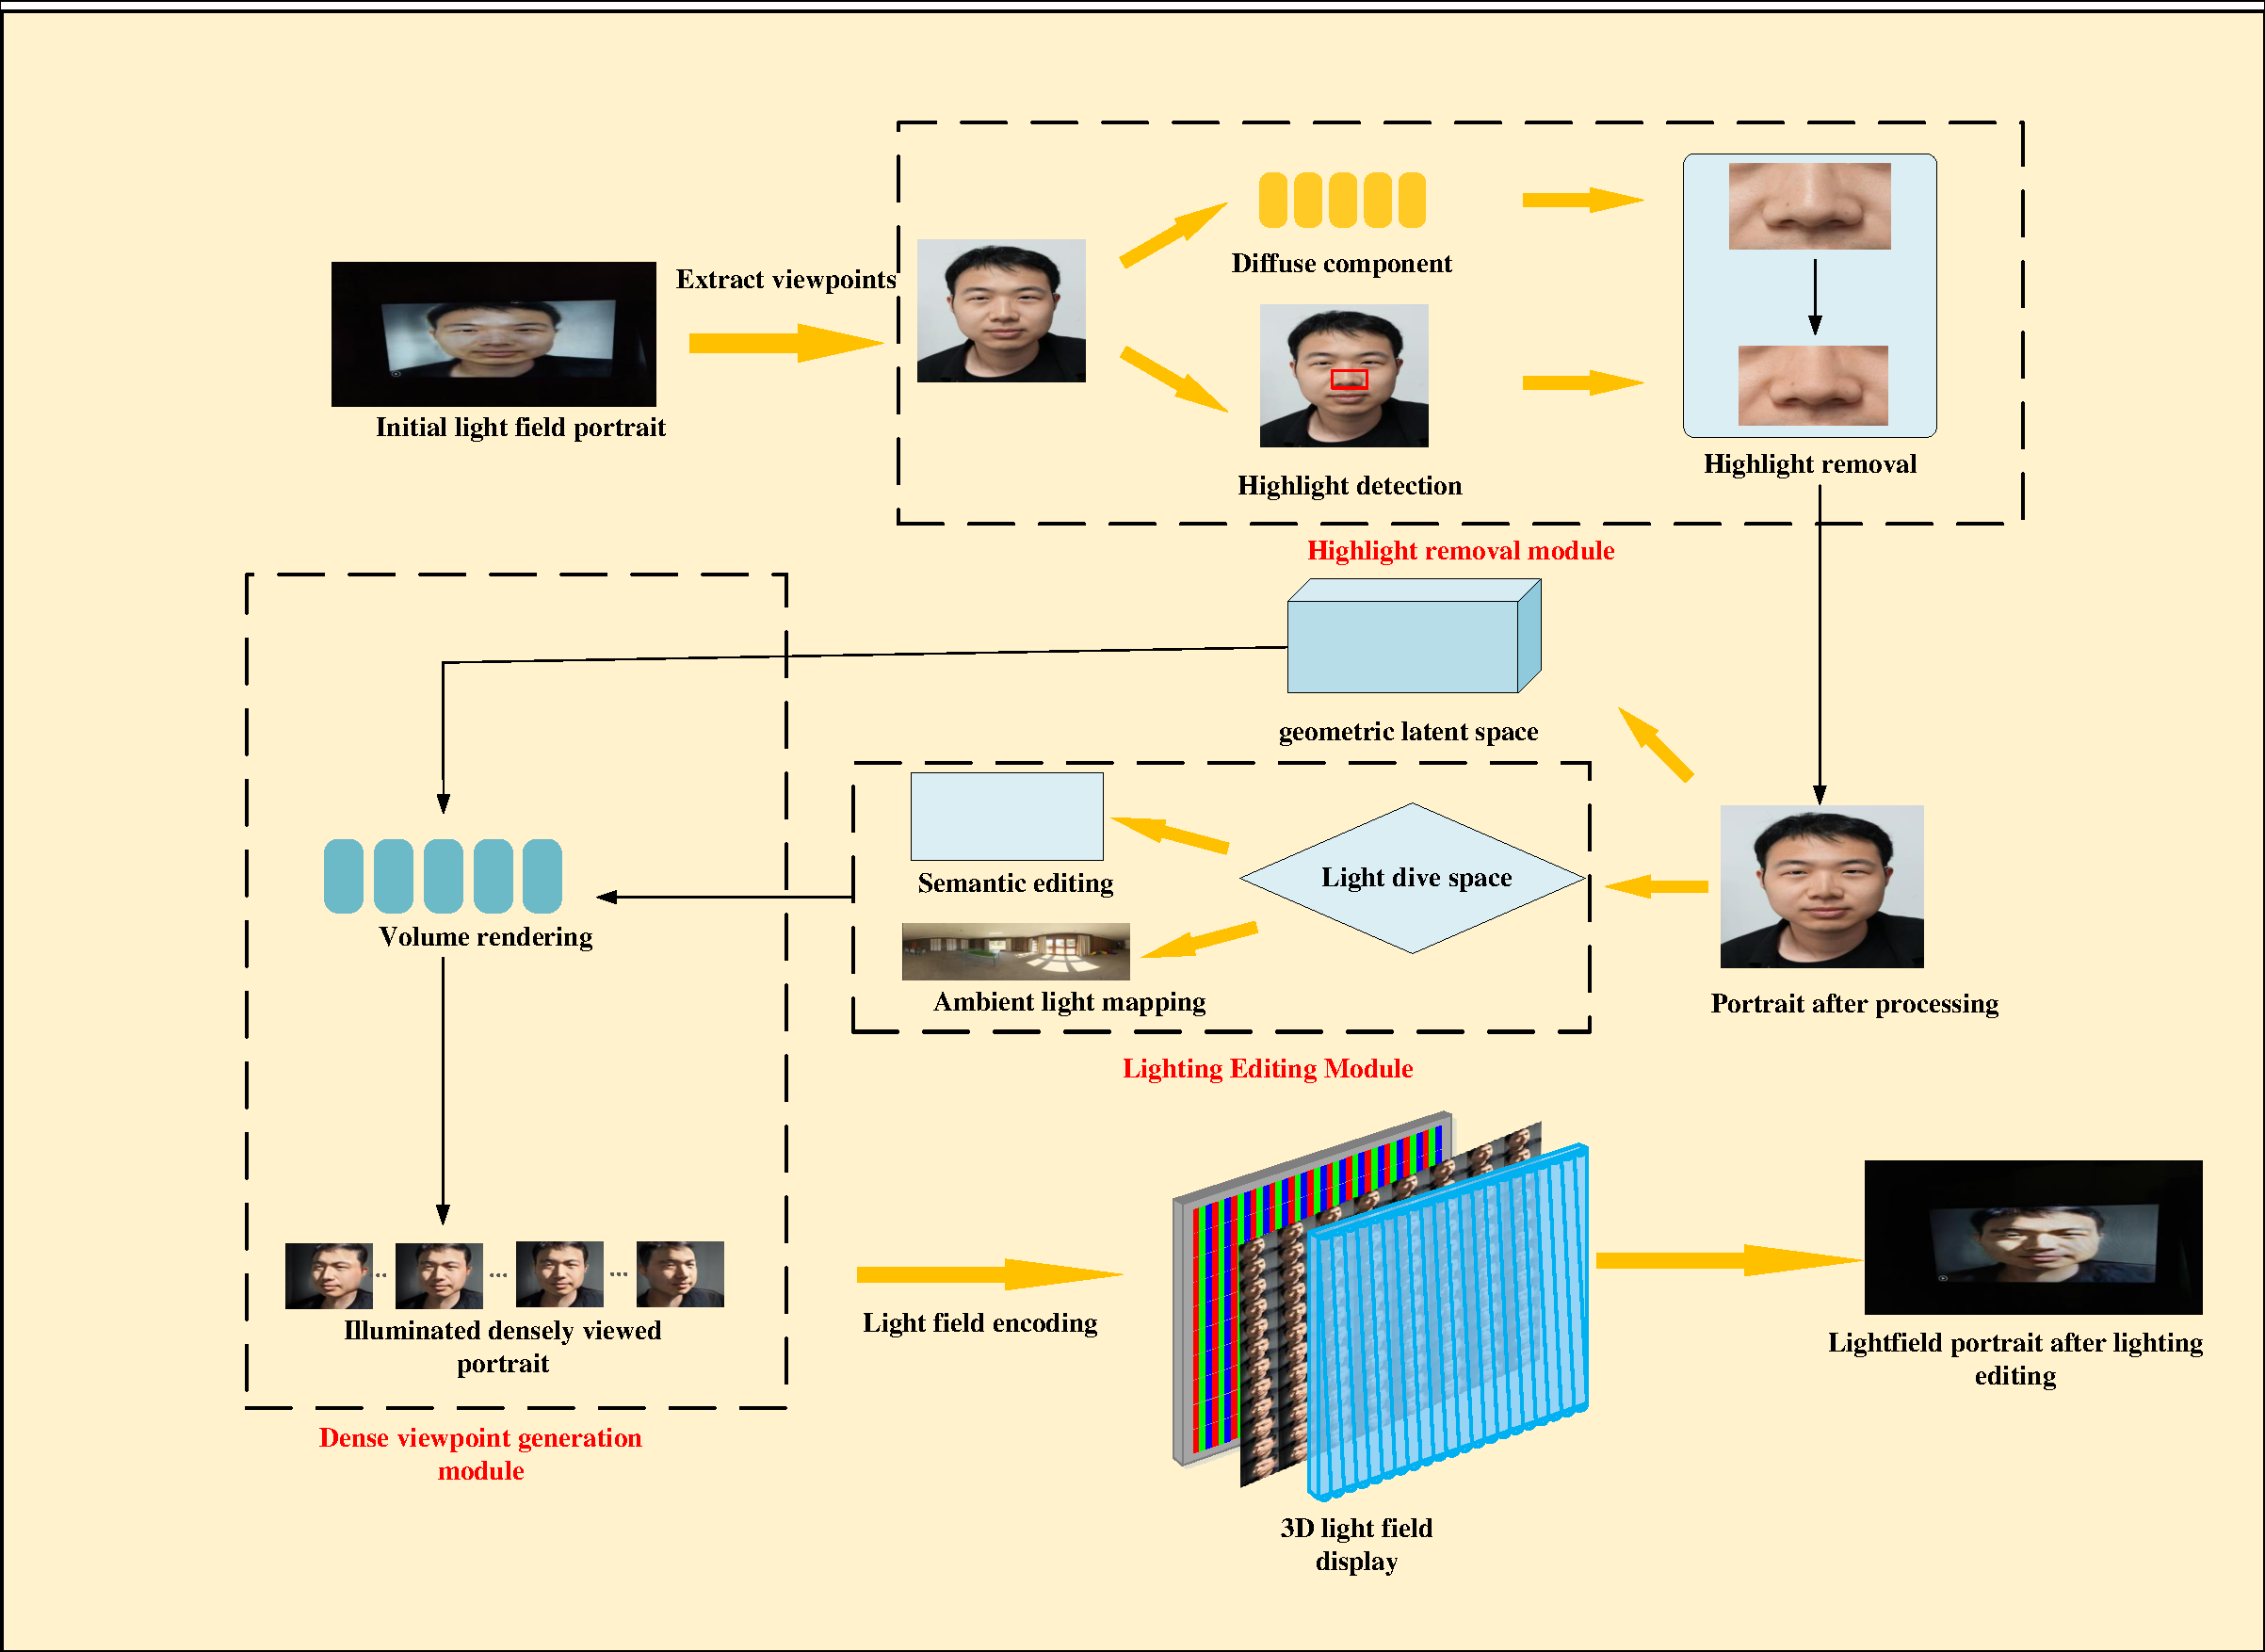
\includegraphics[width=0.8\textwidth,height=12cm]{resources/3p/3-1.pdf}
  % \bicaption{中文标题}{English Caption} % 使用中英文标题
  \caption{总体流程图} % 只使用中文标题
  \label{fig:3-1}
  %\vspace{1 cm} % 使用该指令调整上下间距
\end{figure}

具体而言，该方法由三个部分构成，分别是：高光去除模块，光照编辑模块和密集视点生成模块。

高光去除模块：针对抽取的单张人像图像，采用高光去除算法对原始光照进行预处理。 
由于人像图像的高光区域会因镜面反射导致局部亮度异常，会严重干扰后续三维重建的准确 性。该步骤旨在消除图像中高光区域对后续重建过程的干扰，结合漫反射和亮度阈值来检测 高光区域，并通过像素替换来消除高光，最后得到没有高光区域的人像图片。光照编辑模块：这一环节是实现自定义光照效果的核心所在，其通过双路径编辑策略实现任意环境光渲染与人像光照的语义化编辑。在环境光渲染路径上，运用球面调和（SH）系数计算方法，将 HDR 图像蕴含的复杂光照信息转化为 SH 系数。在人像光照语义化编辑路径上，先提取人像原始光照的 SH 系数，结合语义编辑技术，构建出可解释性强的光照属性调控模型。实现语义化的对光照方向、强度等属性的操作。通过双路径的光照编辑策略，可以满足多样化的场景需求。密集视点生成模块：基于优化后的光照关键信息，引入体渲染技术进行三维重建。输入相机参数，结合光照 SH 系数生成不同视角下的具有自定义光照效果的密集视点人像图像，最后通过光场编码后在三维光场上进行展示。

\subsection{高光去除模块}

\begin{figure}[htbp]
  \centering
  %\vspace{1 cm} % 使用该指令调整上下间距
  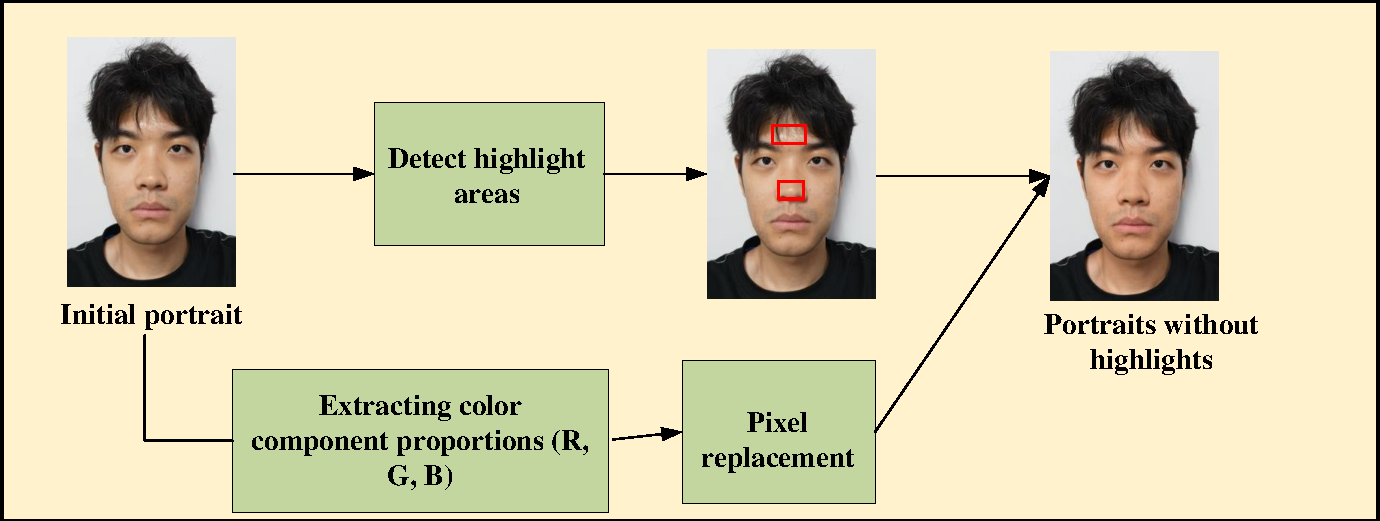
\includegraphics[width=0.8\textwidth]{resources/3p/3-2.pdf}
  % \bicaption{中文标题}{English Caption} % 使用中英文标题
  \caption{高光去除模块} % 只使用中文标题
  \label{fig:3-2}
  %\vspace{1 cm} % 使用该指令调整上下间距
\end{figure}

人像图像中，高光区域的形成源于镜面反射效应，这一现象会引发局部亮度的异常波动，进而对后续三维重建的精度产生显著干扰。为解决后续三维重建过程中的高光干扰问题，本文通过引入高光去除模块来对抽取的单张人像图像实施高光去除预处理。该模块采用高光局部去除算法对人像展开针对性处理。结合漫反射特性与亮度阈值参数构建高光区域检测机制，该双重检测机制可以精准定位图像中的高光区域，随后通过像素替换技术对已检测到的高光区域进行修正，最终输出无高光干扰的人像图像，为后续三维重建流程的顺利进行奠定基础。

高光去除模块分布两个步骤，第一步是亮度阈值检测高光区域，第二步是高光像素替换。具体流程如图\ref{fig:3-2}所示。通过检测高光区域，进行像素替换从而达到去除高光的效果。

1.	双重标准检测高光区域

本文提出一种基于双重检测标准的高光区域定位方法，通过联合亮度阈值筛选与漫反射分量偏移校验，排除了白色物体的高光误判。该设计的核心理论依据来源于双色反射模型\cite{Shafer1985}与动态亮度阈值设计\cite{蔡慧2009}。首先计算当前人像图像的三通道颜色比例，如公式\eqref{eq:2-1}所示，

\begin{equation}
\label{eq:2-1}
(r, g, b) = \left( \frac{R}{R+G+B}, \frac{G}{R+G+B}, \frac{B}{R+G+B} \right)
\end{equation}

其中，\((r, g, b)\)代表红绿蓝三通道颜色在每一个像素块儿的占比，根据双色反射模型，图像亮度可以分解为漫反射分量和镜面分量的线性叠加，其中镜面反射分量在高光区域权重显著增大。通过计算镜面反射的亮度突变特性，可能误判高亮物体（如白色陶瓷）。因此使用双重检测标准来判定高光区域。设置了高光检测的双重条件，超过了设计的阈值V并且颜色比例偏离漫反射分量会被定义为高光区域，这种双重判断标准主要是避免在处理亮度较高的图像时出现的误判问题。比如白色的杯子，亮度就超过阈值，但不是高光。对于阈值V，本文采用“均值+1.2倍标准差”的阈值策略来自适应生成阈值V，其理论依据来自于目标检测领域 ATSS 算法\cite{Zhang2020}中“均值与标准差联合决策”的思想，该方法在多个数据集上证明了对阈值自适应的有效性。具体实现是通过引入MTCNN算法\cite{Zhang2016}进行人脸区域检测与肤色样本提取，计算肤色样本中的三通道颜色的最大值 \(v_i\)，统计出 \(v_i\) 的均值 \(\mu\) 与标准差 \(\sigma\)，通过公式 \eqref{eq:2-2} 得到作为全局阈值 \(V\)：
\begin{equation}
\label{eq:2-2}
V = \mu + 1.2 \times \sigma
\end{equation}

然后由公式 \eqref{eq:brightness_threshold} 计算出人脸区域亮度阈值 \(v\)，\(v\) 代表三通道颜色中占比最大的三原色。
\begin{equation}
\label{eq:brightness_threshold}
v = \max(r, g, b)
\end{equation}

将 \(v\) 与 \(V\) 进行比较，过滤出 \(v > V\) 的像素块，最后再对这些像素块进行漫反射分量基准值校验，设置合适的偏移量 \(\delta\)，通过公式 \eqref{eq:highlight_detection} 计算出偏移量大于 \(\delta\) 的像素，即为高光区域。
\begin{equation}
\label{eq:highlight_detection}
|r - r_i| + |g - g_i| + |b - b_i| > \delta
\end{equation}

其中，\((r_i, g_i, b_i)\) 代表当前像素块所在区域在没有高光时应该具有的基准颜色比例。本文通过引入基于统计肤色模型的人脸处理\cite{Kakumanu2007} 来得到的人像基准颜色比例。

2.高光像素替换

在精准定位高光区域后，本文提出一种动态窗口自适应替换算法，通过邻域非高光像素信息重建被镜面反射污染的像素，来达到去除高光的目的。该方法的核心理论建立在局部平滑先验\cite{Buades2005}与自适应采样准则\cite{Efros1999}之上，具体流程如下：

在得到高光区域的像素块儿之后，进行像素替换即可得到去除高光后的图像。使用动态窗口进行高光替换，如公式 \eqref{eq:highlight_replacement} 所示，
\begin{equation}
\label{eq:highlight_replacement}
\begin{aligned}
R_{new} &= \frac{\sum_{(m,n)} R_{(m,n)}}{N} \\
G_{new} &= \frac{\sum_{(m,n)} G_{(m,n)}}{N} \\
B_{new} &= \frac{\sum_{(m,n)} B_{(m,n)}}{N}
\end{aligned}
\end{equation}

其中，\(R_{new}\) 代表在使用周围非高光像素的平均值替换后得到的新像素值，也就是没有高光干扰的像素。\(G_{new}\) 和 \(B_{new}\) 同理。

根据自适应采样准则来动态调整窗口大小，默认使用 \(3 \times 3\) 的窗口进行替换，计算出窗口里面的非高光区域的像素平均值，然后替换高光区域得到新的像素值。如果高光区域过大，\(3 \times 3\) 的窗口全是高光区域，则对窗口进行动态扩充到 \(5 \times 5\) 或者 \(7 \times 7\)，直到区域内有非高光像素为止，最后得到信息重建后的无高光人像。为后续光照编辑和人像重建打下基础。

\subsection{光照编辑模块}
在计算机图形学领域，精确模拟和编辑环境光照对于实现逼真的场景渲染至关重要。球面调和系数（SH）作为一种高效的光照表示方法，能够将复杂的环境光照信息紧凑地编码为一系列系数。通过计算从环境光高动态范围（HDR）图像中获取 SH 系数，从而达到使用环境光来进行重光照或者直接对光照进行编辑的效果。

1.通过环境光对人像进行重光照

根据帕塞瓦尔定理，自然光照的辐射能量主要分布于低频分量，这一特性使得9个低阶参数就足以近似在保留主要光照特征的同时，显著降低计算复杂度。为了保证重建过程不会过于复杂，又可以真实的还原光照的信息，故本文提出了一种光照编辑方法，选用了前2阶系数，一共9个SH系数来模拟光照。图\ref{fig:3-3}展示了从环境光高动态范围（HDR）图像中获取 SH 系数，进行渲染后展示在三维光场上展示的效果，由于拍摄的照片为2维的，难以表示出3D显示器所展示的立体效果，故从3个角度分别拍摄同一场景，从而得到3张图片来展示其立体效果。
\begin{figure}[htbp]
  \centering
  %\vspace{1 cm} % 使用该指令调整上下间距
  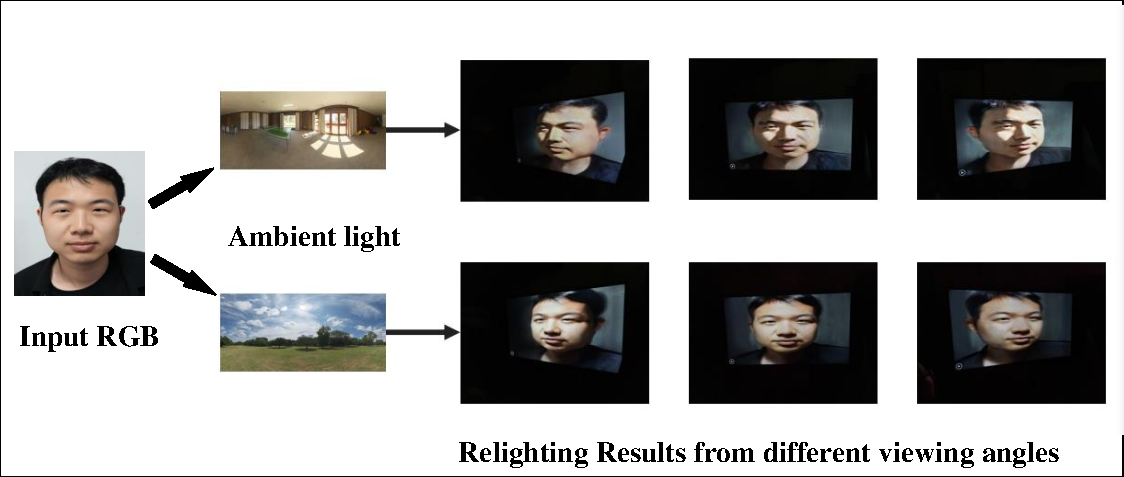
\includegraphics[width=0.8\textwidth]{resources/3p/3-3.pdf}
  % \bicaption{中文标题}{English Caption} % 使用中英文标题
  \caption{环境光重光照} % 只使用中文标题
  \label{fig:3-3}
  %\vspace{1 cm} % 使用该指令调整上下间距
\end{figure}
2.通过语义编辑人像进行光照编辑

针对环境光照的交互式编辑需求，本节提出一种面向整体亮度调节与四方向（左、右、上、下）光照控制的简易方法，通过建立自然语言语义与低阶球面调和（SH）系数的直接映射关系，实现直观高效的光照编辑。通过引入现成的自然语言处理模型BERT\cite{Devlin2019}，将用户输入的自然语言指令（例如 “增加左侧光照”“减弱顶部光源强度” 等）作为模型的输入。

该模型经过预训练已具备较强的语义理解能力，能够精准解析指令中包含的光照方向、强度变化等关键信息。模型的输出被设定为 9 个球谐函数系数，这 9 个系数可有效表征三维空间中的光照分布特性。当输入 “增加左侧光照” 这类指令时，模型会自动识别 “左侧” 对应的空间方位，并通过增大该方位所对应的 SH 系数，实现对人像左侧光照强度的针对性增强。整个实现框架如图\ref{fig:3-4}所示。首先，系统接收自然语言指令，如 “增强右侧光照”，“降低整体亮度”。随后，语义解析模块提取指令中的关键信息，明确调整方向和操作类型，系数映射模块根据预设规则，定位对应的 SH 系数并计算调整量，然后对 SH 系数矩阵进行调整。最后得到调整后的SH系数，用于后续密集视点生成模块中的使用。


\begin{figure}[htbp]
  \centering
  %\vspace{1 cm} % 使用该指令调整上下间距
  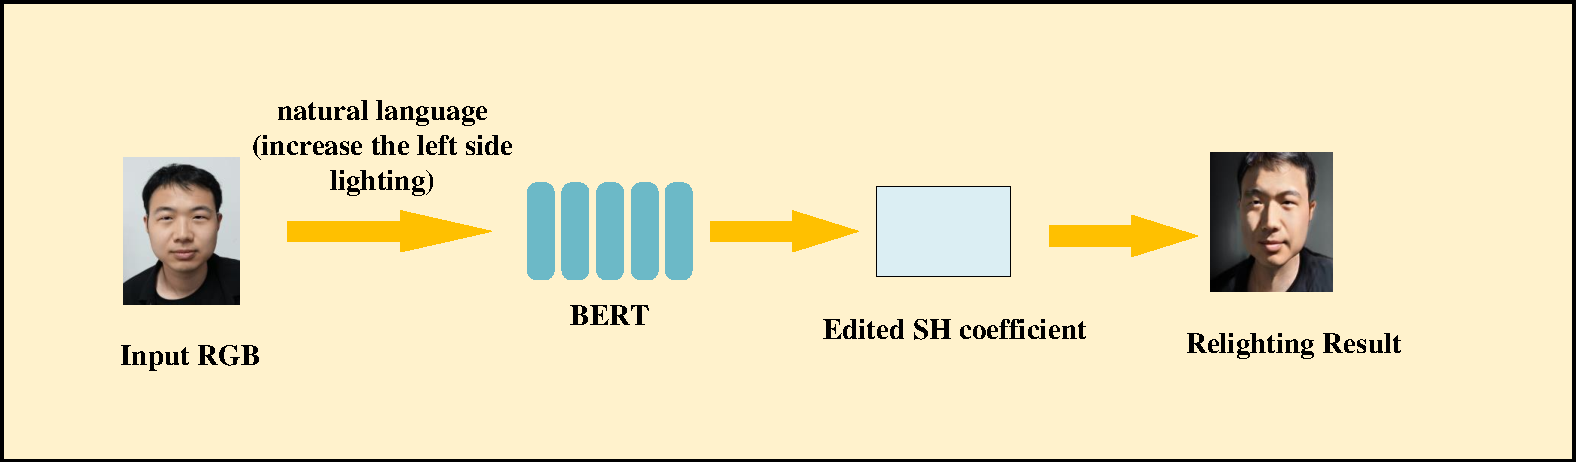
\includegraphics[width=0.8\textwidth]{resources/3p/3-4.pdf}
  % \bicaption{中文标题}{English Caption} % 使用中英文标题
  \caption{语义编辑} % 只使用中文标题
  \label{fig:3-4}
  %\vspace{1 cm} % 使用该指令调整上下间距
\end{figure}


\subsection{密集视点生成模块}
在密集视点生成模块中，将垂直视角恒定设置为 0°，在水平 ±30°的视角范围内，按照特定的采样策略均匀采集 90 个视角数据。本文引入NerfLighting框架，通过输入抽取的单张光场视差图，渲染得到模型，最后生成指定光照条件的密集人像视点。

具体来说，对于空间点 $(x, y, z)$，通过双线性插值投影到三个平面，得到特征向量如公式 \eqref{eq:f_sum} 所示：
\begin{equation}
\label{eq:f_sum}
f_{sum} = f_{xy} + f_{yz} + f_{xz}
\end{equation}

使用 MLP 解码器 $\phi$ 来预测密度 $\partial$ 和颜色特征 $a$，如公式 \eqref{eq:mlp_decoder} 所示：
\begin{equation}
\label{eq:mlp_decoder}
\phi(f_{sum}) = (\partial, a)
\end{equation}

使用阴影解码器 $\omega$ 从阴影三平面预测阴影值 $s$，如公式 \eqref{eq:shadow_decoder} 所示：
\begin{equation}
\label{eq:shadow_decoder}
s = \omega(p_{shading})
\end{equation}

得到最终颜色 $c = s \odot a$。沿相机射线积分，生成视差图，如公式 \eqref{eq:ray_integration} 所示：
\begin{equation}
\label{eq:ray_integration}
C(r) = \int_{t_n}^{t_f} T(t) \partial(r(t)) c(r(t), d) dt
\end{equation}

其中：$r$ 表示光线，$t$ 表示沿光线的采样距离，$T(t)$ 为透射率，$\partial(r(t))$ 为体密度，$c(r(t), d)$ 为辐射颜色。

为了在光场上更好的显示3D效果，本文在渲染之后根据预设的采样策略逐步生成精确的视差图。具体是基于离轴模型的视角生成方法，该方法通过调整相机内参，最终生成水平视角60度范围内的90张连续水平视差的512×512 像素的视图序列。如图\ref{fig:3-5}所示，为光场编码与裸眼 3D 显示提供了高质量输入。

\begin{figure}[htbp]
  \centering
  %\vspace{1 cm} % 使用该指令调整上下间距
  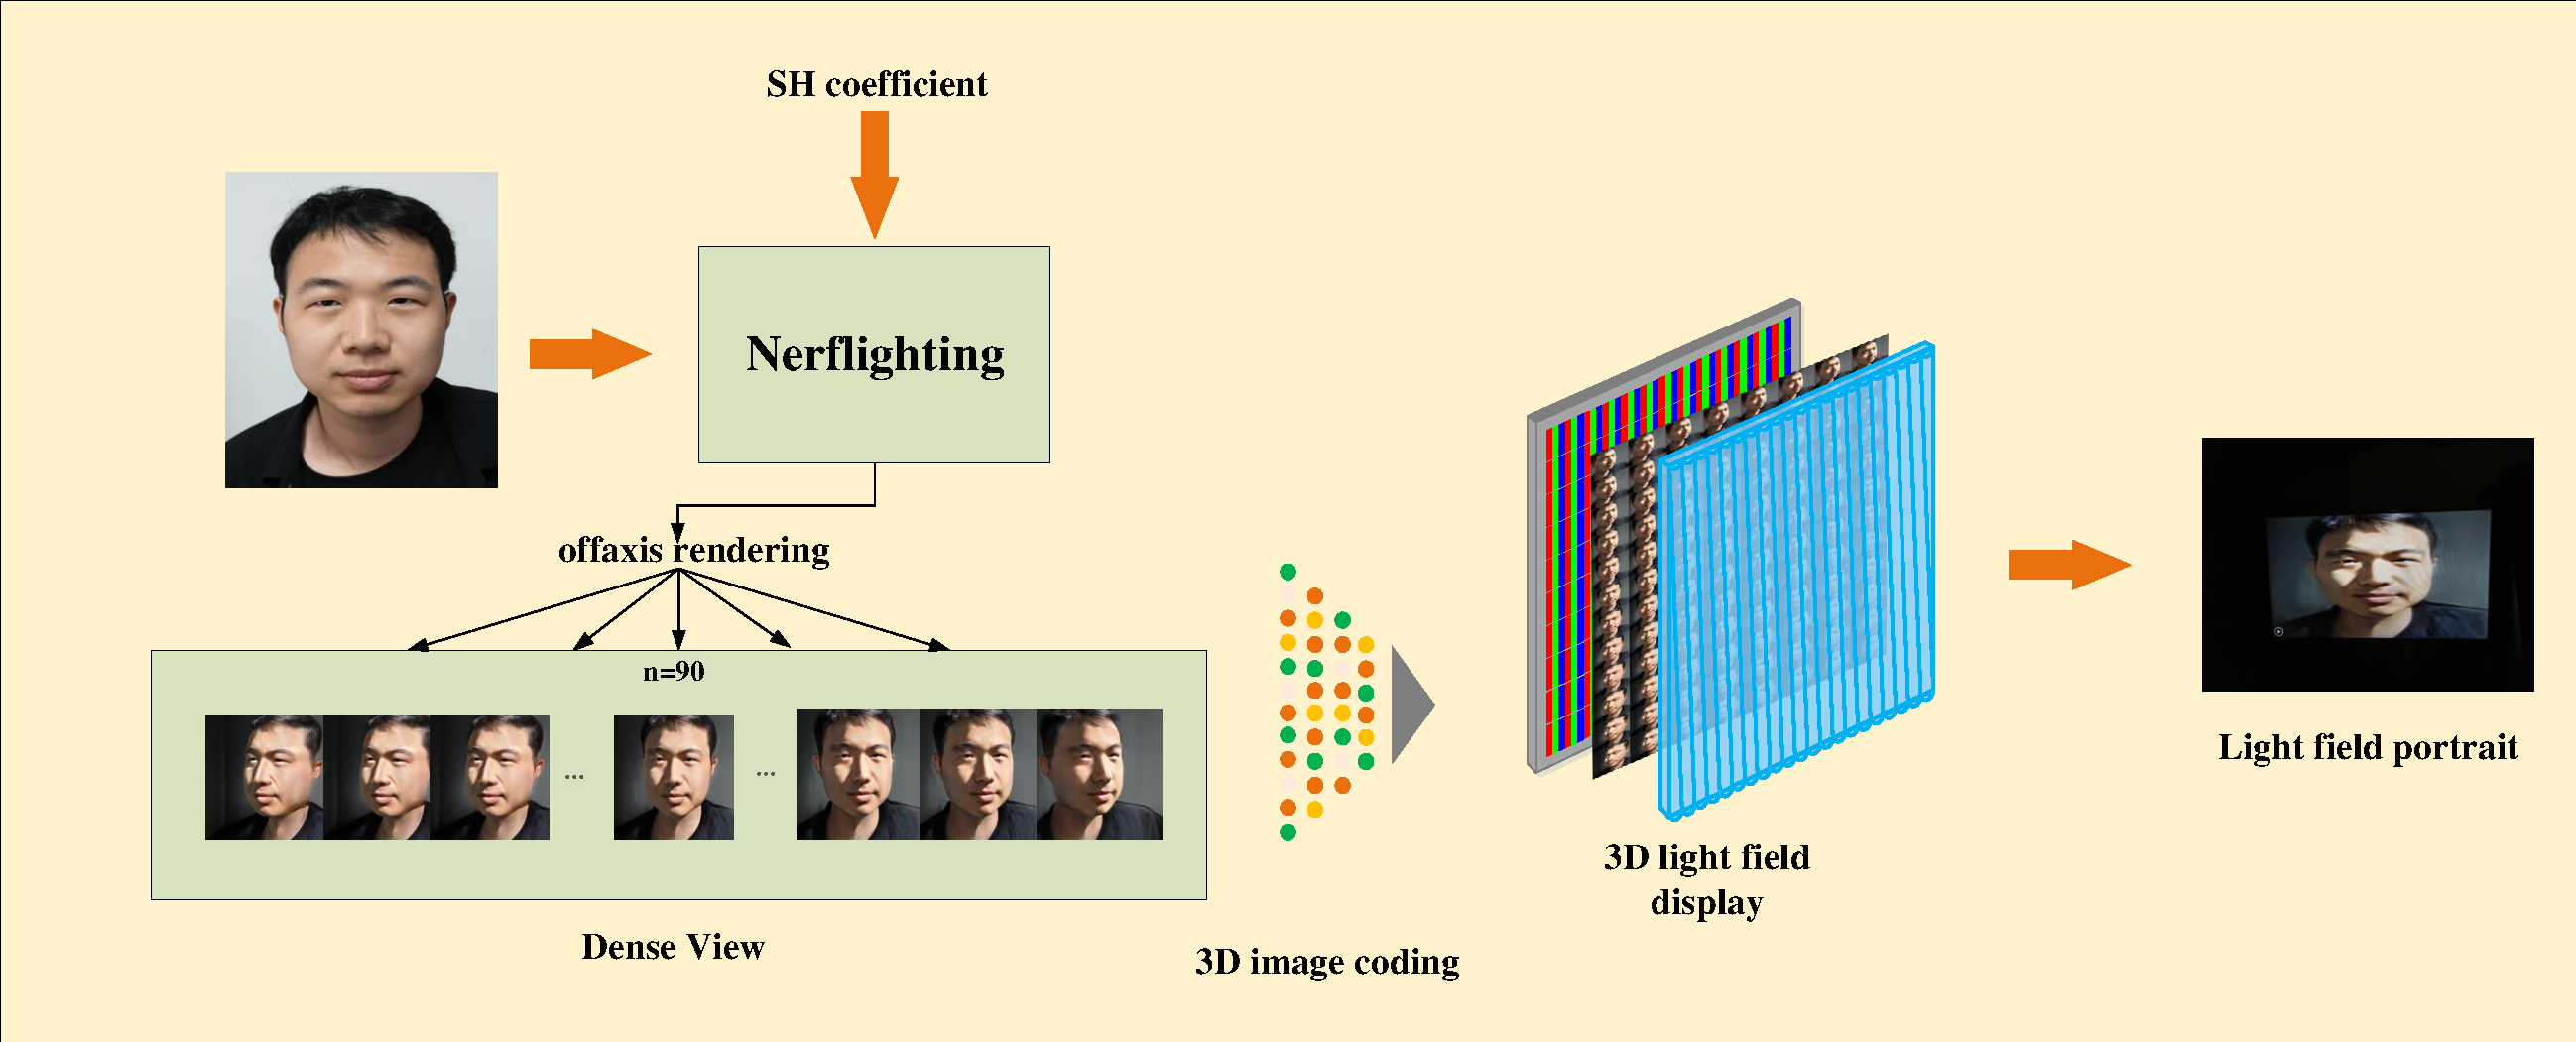
\includegraphics[width=0.8\textwidth]{resources/3p/3-5.pdf}
  % \bicaption{中文标题}{English Caption} % 使用中英文标题
  \caption{光场编码} % 只使用中文标题
  \label{fig:3-5}
  %\vspace{1 cm} % 使用该指令调整上下间距
\end{figure}

\section{实验}
在本节中，将本章提出的方法与当前先进的人像重光照方法进行了对比，并在三维光场上展示比较，进行了客观实验后证明了我们的方法在生成结果方面具有显著优势。为进一步探讨本方法的有效性，最后我们还进行了主观实验，证明了本文方法有助于显著增强3D光场带光照人像的立体感和光照一致性。
\subsection{客观实验结果及分析}
我们将本文的方法进行了定性和定量评估，并将其与如下的人像重光照方法进行了比较：NVPR\cite{Zhang2021}和LRPI\cite{Yeh2022}。

在定性评估中，我们在视觉上比较了本文方法与其他方法的结果。我们将使用本文方法，NVPR和LRPI在3种不同光照条件下生成的3D人像光场图进行了对比。
\begin{figure}[htbp]
  \centering
  %\vspace{1 cm} % 使用该指令调整上下间距
  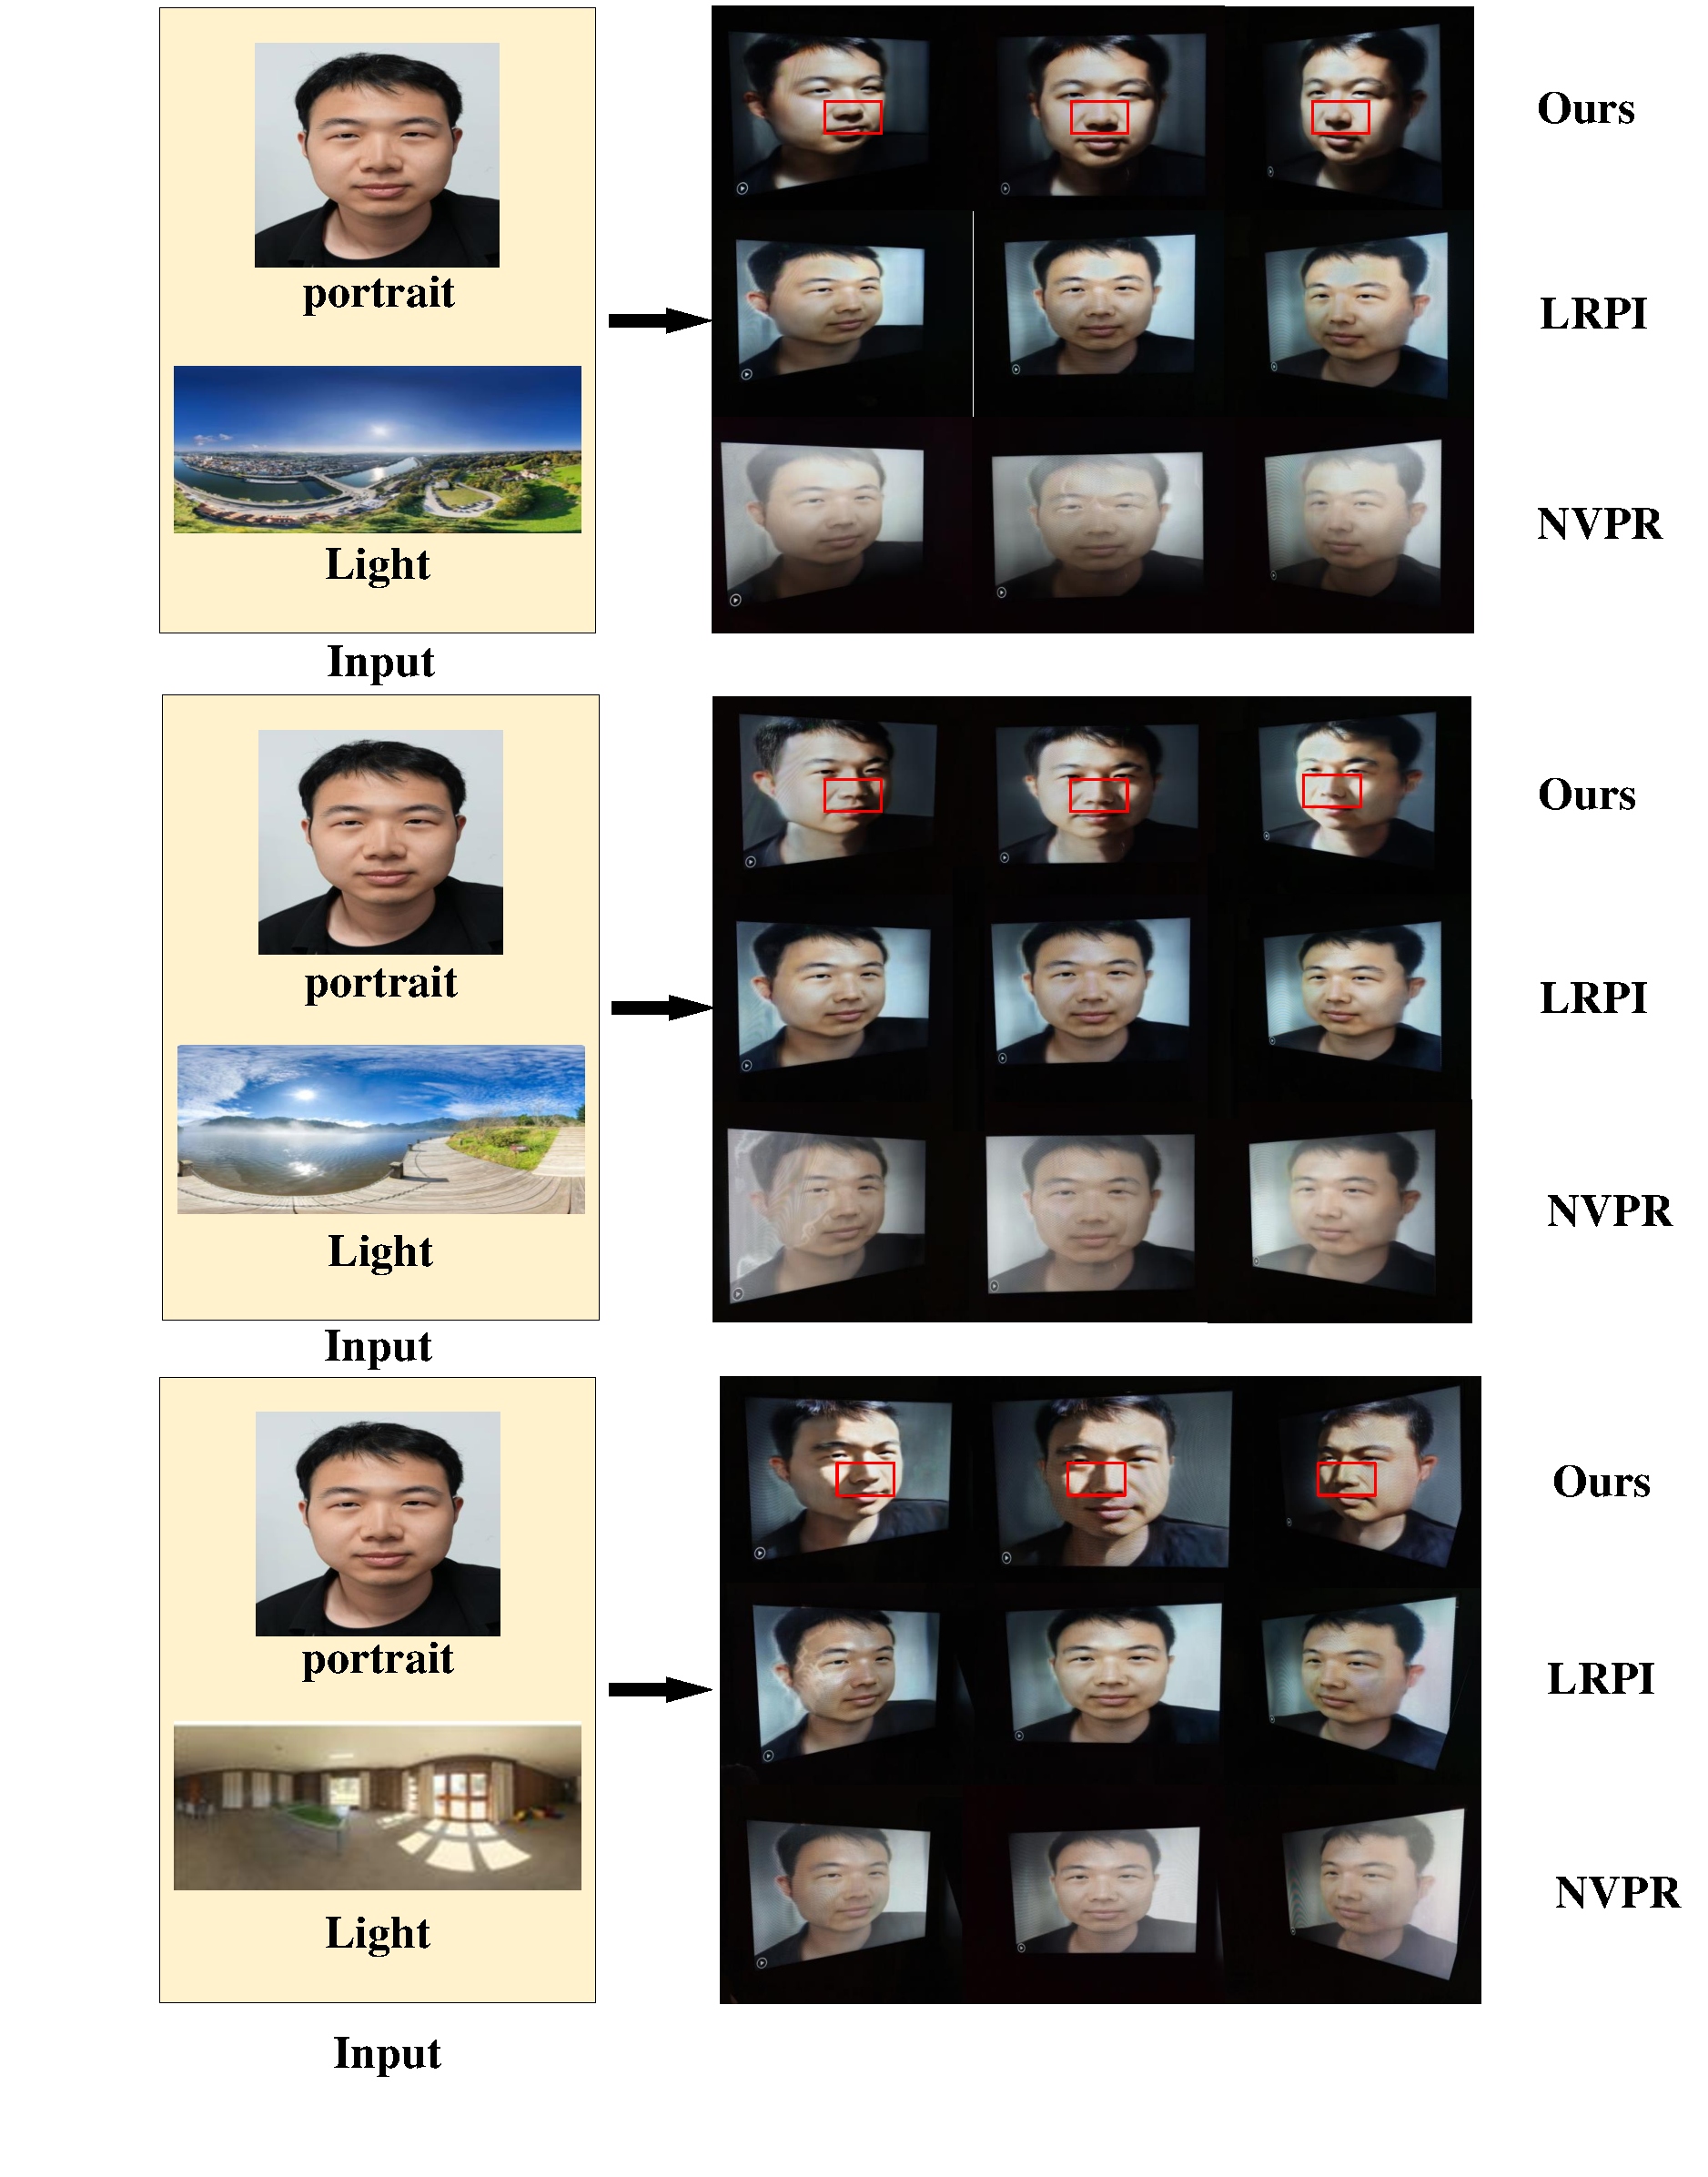
\includegraphics[width=1\textwidth]{resources/3p/3-6.pdf}
  % \bicaption{中文标题}{English Caption} % 使用中英文标题
  \caption{三种不同方法的光场人像对比图} % 只使用中文标题
  \label{fig:3-6}
  %\vspace{1 cm} % 使用该指令调整上下间距
\end{figure}

如图\ref{fig:3-6}所示。通过观察人像受光面的亮度变化是否符合实际光学原理来定性评估重光照的效果优劣。在光照直射处，人像表面应呈现高亮度且高光清晰，而处于阴影区域，亮度应显著降低，且阴影过渡自然，无生硬边界。对比 NVPR、LRPI 及本文方法，若某方法生成的人像光影在明暗分布、高光与阴影位置及形态上，与现实世界中同条件下的人像光照表现更为贴近，便表明其在视觉真实感契合度方面表现更佳。在模拟强烈太阳光下的人像重光照时，本文方法生成的人像面部受光区域亮度高且均匀，鼻梁、额头等突出部位高光精准，阴影从鼻梁、下巴等部位自然过渡，具体细节如图\ref{fig:3-6}红色区域所示。与实际生活中强光下人脸受光情况高度相似，而 NVPR 方法可能出现阴影模糊不清的问题，LRPI 方法存在高光过曝的状况。

直观上可以明显看出，与 NVPR和LRPI方法生成的3D光场图相比，我们的方法得到了更优的重光照结果。本文方法生成的人像存在明确阴影，这归因于我们引入了体渲染框架和隐式光照表示，该方法可以对人像和光照进行解耦，基于双三平面隐式表示捕捉阴影细节，并依托 3D 几何一致性与光照扰动保障阴影真实且泛化，从而呈现明确阴影，精准还原光照关键信息，从而产生更高质量的重光照人像。此外，本文与上述方法相比，本文的数据采集过程更简单、更方便。并且本文的方法具有从任意视点和光照条件下生成图像的能力，这使得本文的方法在应用于3D光场显示时具有优势。

在光场上能够生成更真实自然的光场人像之外，本文方法还可以对光照强度进行精细化的控制，以图\ref{fig:3-7}的效果为例，该方法可在保持人像身份、姿态不变的前提下，对人像右侧光照强度进行阶梯式增强：从初始的柔和侧光，到逐步提升光照能量，再到高光照强度下，整个过程中光照与阴影的过渡始终符合物理规律，无生硬断层或失真，充分验证了该方法在光照编辑上的鲁棒性和适应性。

\begin{figure}[htbp]
  \centering
  %\vspace{1 cm} % 使用该指令调整上下间距
  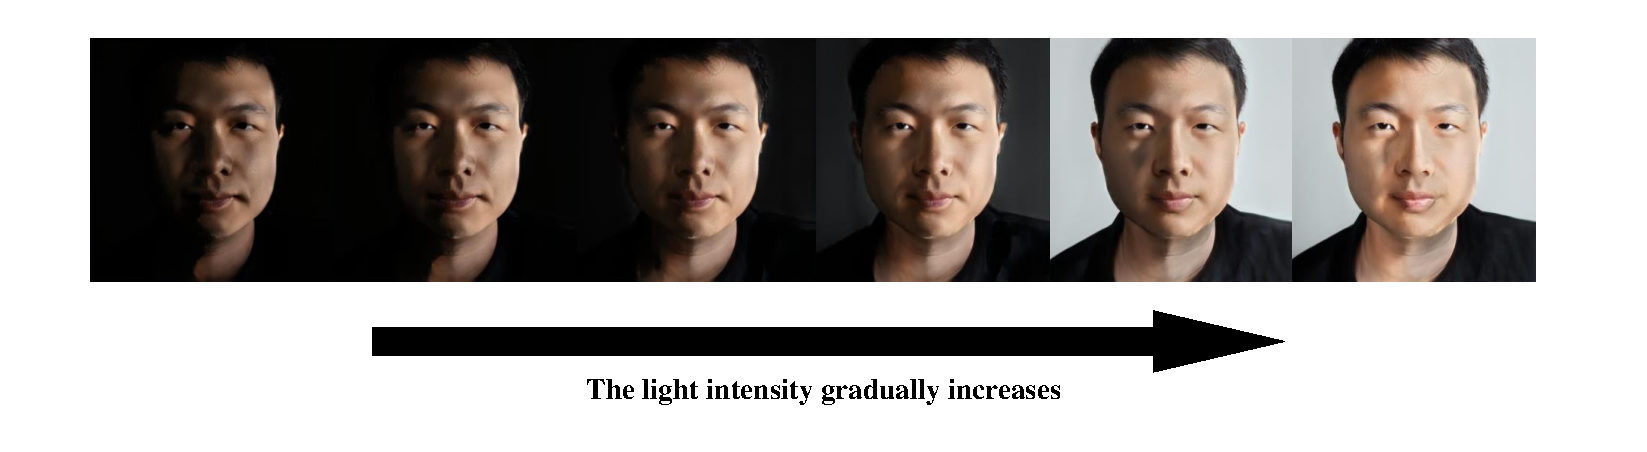
\includegraphics[width=1\textwidth]{resources/3p/3-7.pdf}
  % \bicaption{中文标题}{English Caption} % 使用中英文标题
  \caption{逐步增强人像右侧光照的对比图} % 只使用中文标题
  \label{fig:3-7}
  %\vspace{1 cm} % 使用该指令调整上下间距
\end{figure}

为了评估从输入环境图传递光照信息到重光照结果的准确性，我们从重光照图像中估计光照信息，并将其与目标光照（来自环境图的光照信息）进行比较。具体来说，我们计算了从估计 SH 系数得到的球形渲染图的平均强度，以获得一个全局标量，使其与从目标 SH 系数得到的球形渲染图的平均强度相匹配。我们通过计算重建的球形渲染图与目标球形渲染图之间的 L1 像素差异来衡量准确性。我们的结果显示出更优的数值精度，并且更接近环境图的球形渲染图。

在定量评估中，我们采用客观指标来评估方法的性能。我们使用了以下指标：

Fréchet Inception Distance(FID)：基于深度卷积神经网络特征衡量图像集之间的相似性（值越低越好）。Peak Signal-to-Noise Ratio (PSNR)：通过比较最大信号功率与噪声来指示图像保真度（值越高越好）。Structural Similarity Index (SSIM)\cite{Heusel2017}：基于感知的模型，评估亮度、对比度和结构相似性（值越高越好）。Learned Perceptual Image Patch Similarity (LPIPS)\cite{Zhang2018}：基于深度神经网络特征评估感知相似性（值越低越好）。本文的方法获得了较低的 FID 和 LPIPS 分数，以及较高的 PSNR 和 SSIM 值，表明生成图像与真实图像（Ground Truth）之间具有更高的相似性和图像质量，如表\ref{tab:3-1}所示。我们随机选择了10张图像来提取光源信息作为重光照的目标照明，其中，这10张真实图像均来自于实拍采集的人像数据。随后，我们基于此目标照明生成结果，并使用 FID、PSNR、SSIM 和 LPIPS 等指标进行比较。最后，我们计算平均值得到结果。我们的方法在这些指标上始终取得了更高的分数，表明其具有更好的重建质量且更接近真实图像。

\begin{table}[htbp]
  \centering
  \caption{同一观看视角下与前两种方法的指标对比}
  \label{tab:3-1}
  \small
  \begin{tabular}{lccccc}
    \toprule
    Method & Lighting $\downarrow$ & FID $\downarrow$ & PSNR $\uparrow$ & SSIM $\uparrow$ & LPIPS $\downarrow$ \\
    \midrule
    NVPR  & -                    & 36.54           & 28.66           & 0.6288          & 0.30             \\
    LRPI  & 0.0654               & 36.15           & 28.44           & 0.8145          & 0.23             \\
    Ours  & 0.0607               & 33.55           & 32.06           & 0.8954          & 0.19             \\
    \bottomrule
  \end{tabular}
\end{table}

我们还测试了该方法光照编辑的推理时间，在单块 NVIDIA RTX 3090 GPU 上，对1K分辨率的静态人脸进行光照编辑的平均耗时如下表所示：

\begin{table}[htbp]
  \centering
  \caption{光照编辑单帧推理时间对比}
  \label{tab:inference_time_3090}
  \begin{tabular}{lccc}
    \toprule
    Method & NVPR    & LRPI    & Ours     \\
    \midrule
    Time(s) $\downarrow$ & 230.45  & 180.21  & 25.92    \\
    \bottomrule
  \end{tabular}
\end{table}

实验结果表明，本文方法在保持更高重建质量和更接近真实图像视觉效果的同时，光照编辑效率也得到了显著提升。

\subsection{主观实验结果及分析}

为进一步探讨本方法的有效性。本文基于三维光场显示器对实验结果进行了主观实验，来对三维光场人像光照编辑的结果进行评价。实验主要分为两个部分，将本文方法编辑得到的三维光场人像和单视图编辑得到的三维光场人像进行对比，主要评估不同光照条件下光场人像的真实度和不同视角下光照一致性的情况。

实验选用了单视图单张依次编辑三维光场人像光照的方法与本方法进行对比，实验分别在三个不同人像的基础上，编辑了包含左侧光照，顶部光照，右侧光照，底部光照四种不同的光照场景，总共是24组三维光场人像场景，编辑好后，进行光场编码，并在三维显示器上进行显示，其中方法A代表本文的方法，方法B代表单视图单张依次编辑三维光场人像光照的方法，主观实验中方法A和方法B生成的部分3D光场人像如图\ref{fig:3-8}所示，其中左侧的图像均来自于实拍采集的人像数据。右侧分别是使用方法A生成的部分三维光场人像场景和使用方法B生成的部分三维光场人像场景。

24组场景，编号为1到24。比如第一组场景里面的使用本文的方法编辑生成的三维光场人像就用1(a)表示。实验参与者进行观看评估。主观实验的参与者中，男性10名，女性10名，视力正常或矫正后正常，无色彩感知障碍，所有参与者都给予了书面知情同意。

\begin{figure}[htbp]
  \centering
  %\vspace{1 cm} % 使用该指令调整上下间距
  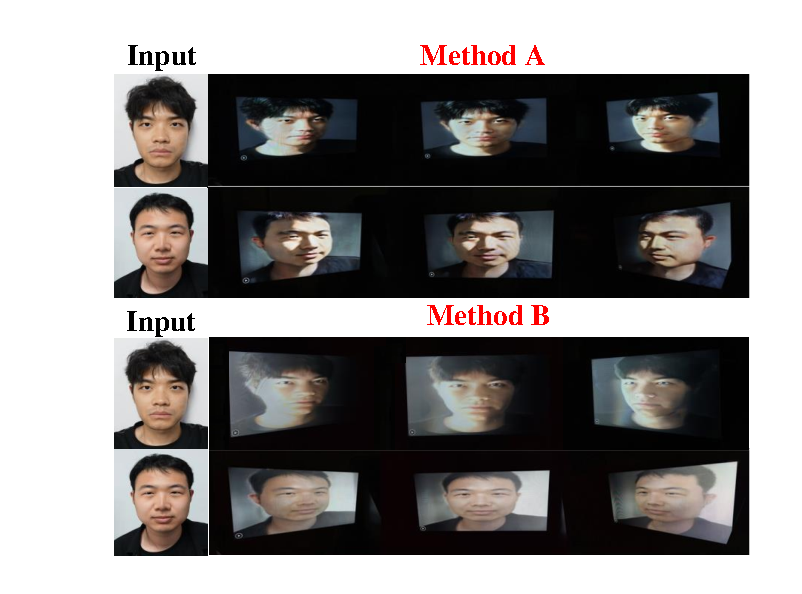
\includegraphics[width=1\textwidth]{resources/3p/3-8.pdf}
  % \bicaption{中文标题}{English Caption} % 使用中英文标题
  \caption{主观实验中方法A和方法B生成的部分3D光场人像} % 只使用中文标题
  \label{fig:3-8}
  %\vspace{1 cm} % 使用该指令调整上下间距
\end{figure}

在主观实验流程中，实验流程如下，实验会将会对24组场景在三维显示器上展示，每一组场景有2个场景，参与者对每一组的两个场景有1分钟时间左右观察，观察后对三维光场人像添加了光照之后的真实感和光照一致性进行评估，比如，第一组我们会依次展示场景1(a)，1(b)两个A，B方法生成相同光照条件的场景。参与者对于每一组场景进行投票，将票投给主观感受上更具有立体感的方法。光照一致性的投票如上，每一个场景最多可以获得20张选票。依次播放完24组场景，整个实验流程大约耗时20分钟。

实验场地如图\ref{fig:3-9}所示，我们使用裸眼3D显示器，参数如表\ref{tab:3-2}所示。

\begin{table}[htbp]
  \centering
  \caption{3D光场的显示参数}
  \label{tab:3-2}
  \small
  \begin{tabular}{lc}
    \toprule
    Display Parameters & Value \\
    \midrule
    Single view resolution & $960 \times 540$ \\
    ColNum & 8 \\
    RowNum & 12 \\
    View number & 96 \\
    Inclined angle & $8.5308^\circ$ \\
    LineNum & 28.08119 \\
    Angle of view & $100^\circ$ \\
    \bottomrule
  \end{tabular}
\end{table}

\begin{figure}[htbp]
  \centering
  %\vspace{1 cm} % 使用该指令调整上下间距
  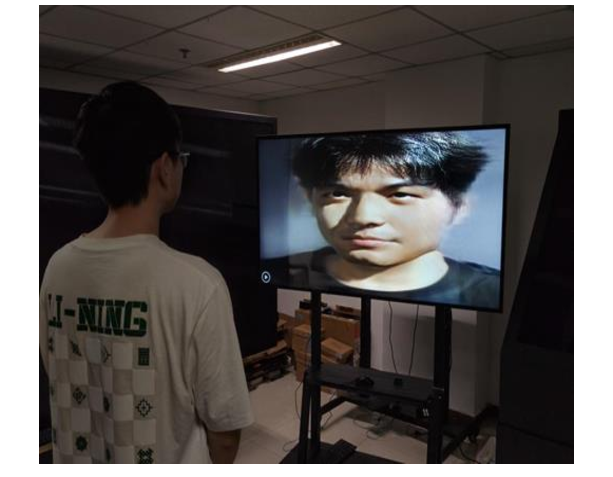
\includegraphics[width=1\textwidth]{resources/3p/3-9.pdf}
  % \bicaption{中文标题}{English Caption} % 使用中英文标题
  \caption{实验场地} % 只使用中文标题
  \label{fig:3-9}
  %\vspace{1 cm} % 使用该指令调整上下间距
\end{figure}

参与者站在距离显示器2米左右位置上进行观察，因为需要观察三维显示器不同视角下的光照一致性情况，参与者在观察时会进行左右的来回走动观察和感受。观察结束后再进行投票，投完票之后再进行下一个场景的观察与投票。为了避免每一组的AB场景会对后续场景的评估产生影响，实验会保证每一组的AB场景的播放顺序是随机的，并且参与者可以反复观看进行对比，同时也减少了惯性思维对实验结果的影响。

为了方便对比，本文提出的方法用后缀A进行表示，单视图依次编辑光照的方法用后缀B表示。通过主观实验对三维光场人像的展示，主要做两个部分的实验，分别是不同参与者对24组场景的立体感的评价结果和不同参与者对24组场景的光照一致性的评价结果。
\begin{figure}[htbp]
  \centering
  %\vspace{1 cm} % 使用该指令调整上下间距
  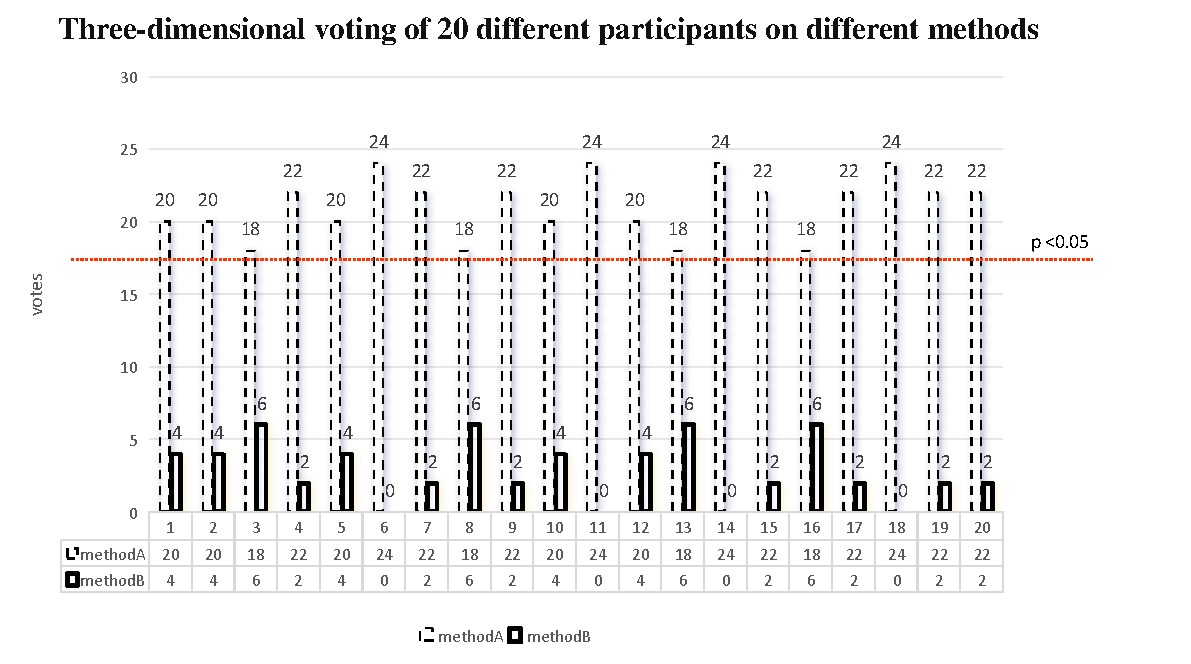
\includegraphics[width=1\textwidth]{resources/3p/3-10.pdf}
  % \bicaption{中文标题}{English Caption} % 使用中英文标题
  \caption{20个不同参与者对不同方法的立体感投票情况} % 只使用中文标题
  \label{fig:3-10}
  %\vspace{1 cm} % 使用该指令调整上下间距
\end{figure}
% \subsubsection{三级标题}

3D立体感的评价结果如图\ref{fig:3-10}所示。假设参与者的投票遵循二项分布 ，对每个场景都应用了二项检验。如果两种方法编辑人像光照后给参与者产生的立体感类似，则投票数预计为总票数中的 1/2。因此，如果某种方法的得票数明显大于此值，说明该方法能够给呈现出更好的3D立体感。

对于图\ref{fig:3-10}所示的结果展示，柱状图统计了所有20名参与者参加24次实验的投票结果汇总，其中，虚线柱代表方法A（本文方法）编辑光照得到的选票数，实线柱代表方法B（单张视图依次编辑三维光场人像）编辑光照得到的选票数，方法A在的3D立体感上的最低得票率为80\%，最高得票率为100\%，平均得票率为88.75\%。假设方法A和方法B对参与者呈现的3D视觉立体感类似，在统计意义上的显著的的得票率为20票（n=24 的二项检验，多次比较的 Bonferroni校正\cite{Bonferroni1936}P<0. 05），获得超过20票，在图10中已经划线表示，即可否定原假设，认为票数更多的方法能够呈现更好的3D立体感，在20名参与者中，有16名参与者认为方法A编辑后的到的三维光场人像的3D立体感更佳。
\begin{figure}[H]
  \centering
  %\vspace{1 cm} % 使用该指令调整上下间距
  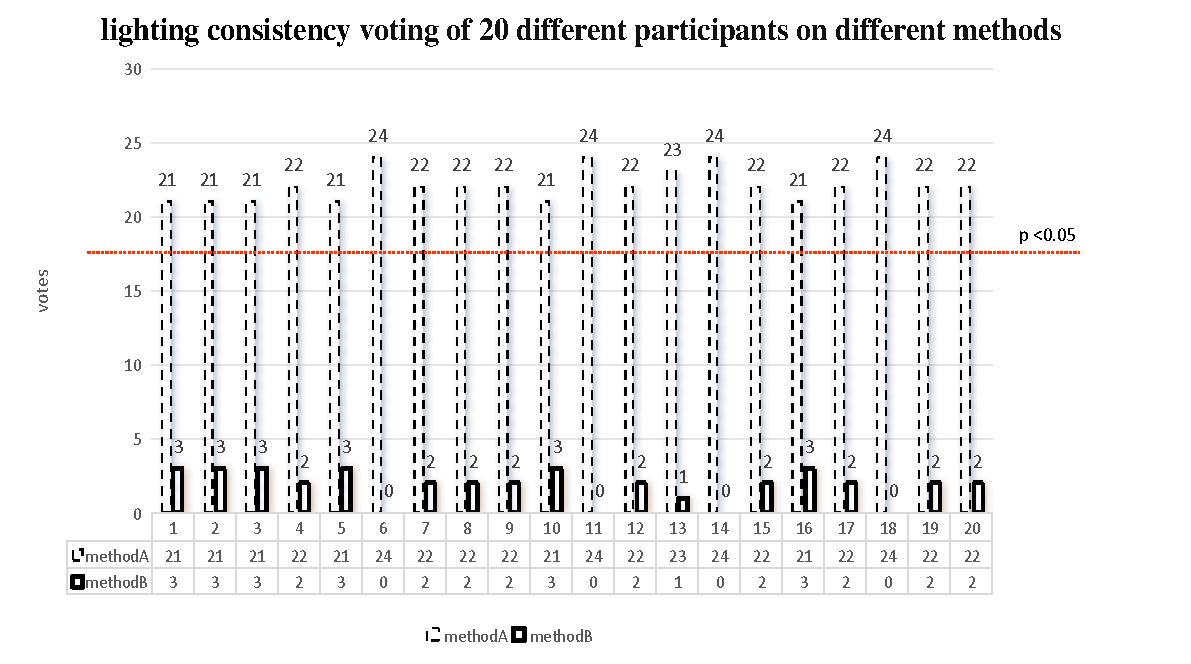
\includegraphics[width=1\textwidth]{resources/3p/3-11.pdf}
  % \bicaption{中文标题}{English Caption} % 使用中英文标题
  \caption{20个不同参与者对不同方法的光照一致性投票情况} % 只使用中文标题
  \label{fig:3-11}
  %\vspace{1 cm} % 使用该指令调整上下间距
\end{figure}

光照一致性的评价结果如图\ref{fig:3-11}所示。参与者在指导下通过左右移动观察3D显示器展示的内容，然后根据主观感受来投票选出不同视角下光照一致性更强的场景。假设参与者的投票遵循二项分布 ，对每个场景都应用了二项检验。如果两种方法编辑人像光照后给参与者产生的光照一致性类似，则投票数预计为总票数中的 1/2。因此，如果某种方法的得票数明显大于此值，说明该方法能够给呈现出更好的光照一致性。

对于图\ref{fig:3-11}所示的结果展示，柱状图统计了所有20名参与者参加24次实验的投票结果汇总，其中，虚线柱代表方法A（本文方法）编辑光照得到的选票数，实线柱代表方法B（单张试图依次编辑三维光场人像）编辑光照得到的选票数，方法A在的3D立体感上的最低得票率为80\%，最高得票率为100\%，平均得票率为92.29\%。假设方法A和方法B对参与者呈现的光照一致性类似，在统计意义上的显著的的得票率为20票（n=24 的二项检验，多次比较的 Bonferroni校正P<0. 05），获得超过20票，在图11中已经划线表示，即可否定原假设，认为票数更多的方法能够呈现更好的光照一致性，在20名参与者中，所有参与者认为方法A编辑后的到的三维光场人像的光照一致性更佳。
\begin{table}[htbp]
  \centering
  \caption{实验方法得票总数}
  \label{tab:3-3}
  \small
  \begin{tabular}{lc}
    \toprule
    Type of experiment & Total votes \\
    \midrule
    three-dimensional (method A) & 428 \\
    three-dimensional (method B) & 52 \\
    lighting consistency (method A) & 443 \\
    lighting consistency (method B) & 37 \\
    \bottomrule
  \end{tabular}
\end{table}

对于表\ref{tab:3-3}的统计结果，记录了在24组不同场景的20名参与者分别进行两组实验的投票结果汇总。分别是光照一致性实验和立体感实验，方法A(本文的方法),方法B(基于单视图编辑光照的方法)。得票数为这两种方法编辑在这24组场景的背景下，分别从20名参与者身上得到的选票数。统计得到方法A在24组场景下的立体感得票率为89.19\%，方法B的平均得票率为10.81\%。假设方法A编辑三维光场人像光照后的立体感没有提升，那统计结果三种方法的得票率应在50\%上下浮动。证明了使用本文方法编辑光场人像光照后，立体感和光照一致性均得到了提升。

\section{本章小结}
本章提出了一种关键信息驱动的三维光场人像光照的编辑方法，该方法通过抽取多视图，通过获取漫反射分量，并结合高光阈值多重判断来去除图像高光，因为三维光场现实内容由多张视差图构成，并且视差图光照不均匀或者存在高光，高光会贴合在人像上，对后续重建效果产生影响，所以先进行光照均匀化处理。然后进行重建，将图像解耦成几何空间和光照潜空间，通过全景 HDR 图像快速获取环境光信息并通过语义级别描述的对光照潜空间的关键信息进行编辑，结合几何空间和光照潜空间，并通过体渲染渲染得到密集视差图，最后在3D显示器上进行显示验证，完成对三维光场人像光照的编辑。

本章进行了客观实验和主观实验，在客观实验中，与当前重光照方法NVPR和LRPI进行了对比，本方法可以生成更自然真实的光照条件，没有出现光线泛白，不同角度光线不一致的问题，在FID、PSNR、SSIM 和 LPIPS 等指标中都取得了更优的分数，并且能够更快的进行静态人像光照编辑。在主观实验中，本文方法和依次对多张视差图进行人像光照的编辑方法进行了实验对比。在立体感上，本方法得票率为89.19 \%，证明了本方法编辑后的人像具有更高的立体感，在光照一致性的投票上，本方法得票率为92.29\%，证明了本方法编辑后的人像具有更好的光照一致性。上述实验证明了该方法在提高了光照一致性的前提下，简单高效的实现对三维光场光照的编辑。本方法还可以通过环境光照来编辑光场人像的光照，并取得了较好效果，并且可以显著增强3D光场带光照人像的立体感和光照一致性，可能成为未来对静态场景3D光场显示进行光照编辑的重要方法。

目前研究工作中仍有不少可改进之处。在拓展至动态人脸视频场景时仍存在明显局限性：面对人脸的连续姿态变化、表情运动，现有框架难以兼顾帧间光照的时序连续性，易出现光照闪烁、高光跳变等问题；同时，多视角光照一致性的约束仅针对单帧静态几何，无法适配动态场景下的跨帧几何形变，导致动态序列的多视角光照出现时空失配。针对上述动态场景的技术痛点，后续工作将聚焦于时间 - 空间双维联合优化，构建专门面向动态人脸的三维光场光照编辑框架，重点解决时序闪烁与动态多视角光照失配问题，实现高质量的动态三维光场人脸光照编辑。


